\documentclass[../Head/Main.tex]{subfiles}
\begin{document}
\section{Photogrammetry}
In this section, our goal is to take the partially overlapping images we got from the drone, and stitch them together.
We aim to get a large, high definition image, that looks like it was taken from a higher altitude, 
capturing a larger land area than any single original image from the set.

To create the orthomosaic, we chose Agisoft Metashape Pro. 
We tried different quality settings and compared the results.

\subsection{Alignment}

The first step, after loading the images in Metashape, is to align them.
The alignment process looks for matching point pairs in multiple images and estimates their relative alignment based on the relative position offset of the point pairs.
We tried three quality options, medium, higher and highest.
The highest quality option failed, but both higher and medium ran successfully.
Both options took around a few seconds and there was no noticable difference in the results.

\subsection{Digital Elevation Model}
The digital elevation model is a 3D representation of a surface.
This can be computed by finding point pairs for each pixel and calculating from the disparity.
Not all pixels have pairs, in which case it can be estimated based on its neighbourhood.
For this computation, we left the default parameters suggested by the program unchanged.

\subsection{Orthomosaic}


IN THIS SECTION SHOULD BE INCLUDED:
\begin{itemize}
\item Bundle adjustment
\item Digitial elevation model
\item Orthorectification and orthomosaic creation
\item EXIF data
\item Number of images and approximate overlap
\item Size of orthomosaic (resolution and disk size)
\item Description of handling outside the fence data (cropping of the image)
\item Screen shots of DSM and orthomosaic

\subsection{Exif data}
The camera used was a senseFly S.O.D.A. with an image resolution of 5472 z 3648 pixels. The type of UAV was not specified by the EXIF informations but it was either a senseFly eBee X or eBee Classic.


senseFly S.O.D.A.\\
Exposure Time : 1/1000\\
Aperture      : 2.8\\
ISO           : 200
Exposure program : AE (exposure priority)
Focal length  : 10.2 mm
Image size    : 5472 x 3648
White balance : Auto
Pitch                           : 6.029021
Roll                            : -7.621159
Yaw                             : 316.127563



\begin{figure}[H]
	\centering
	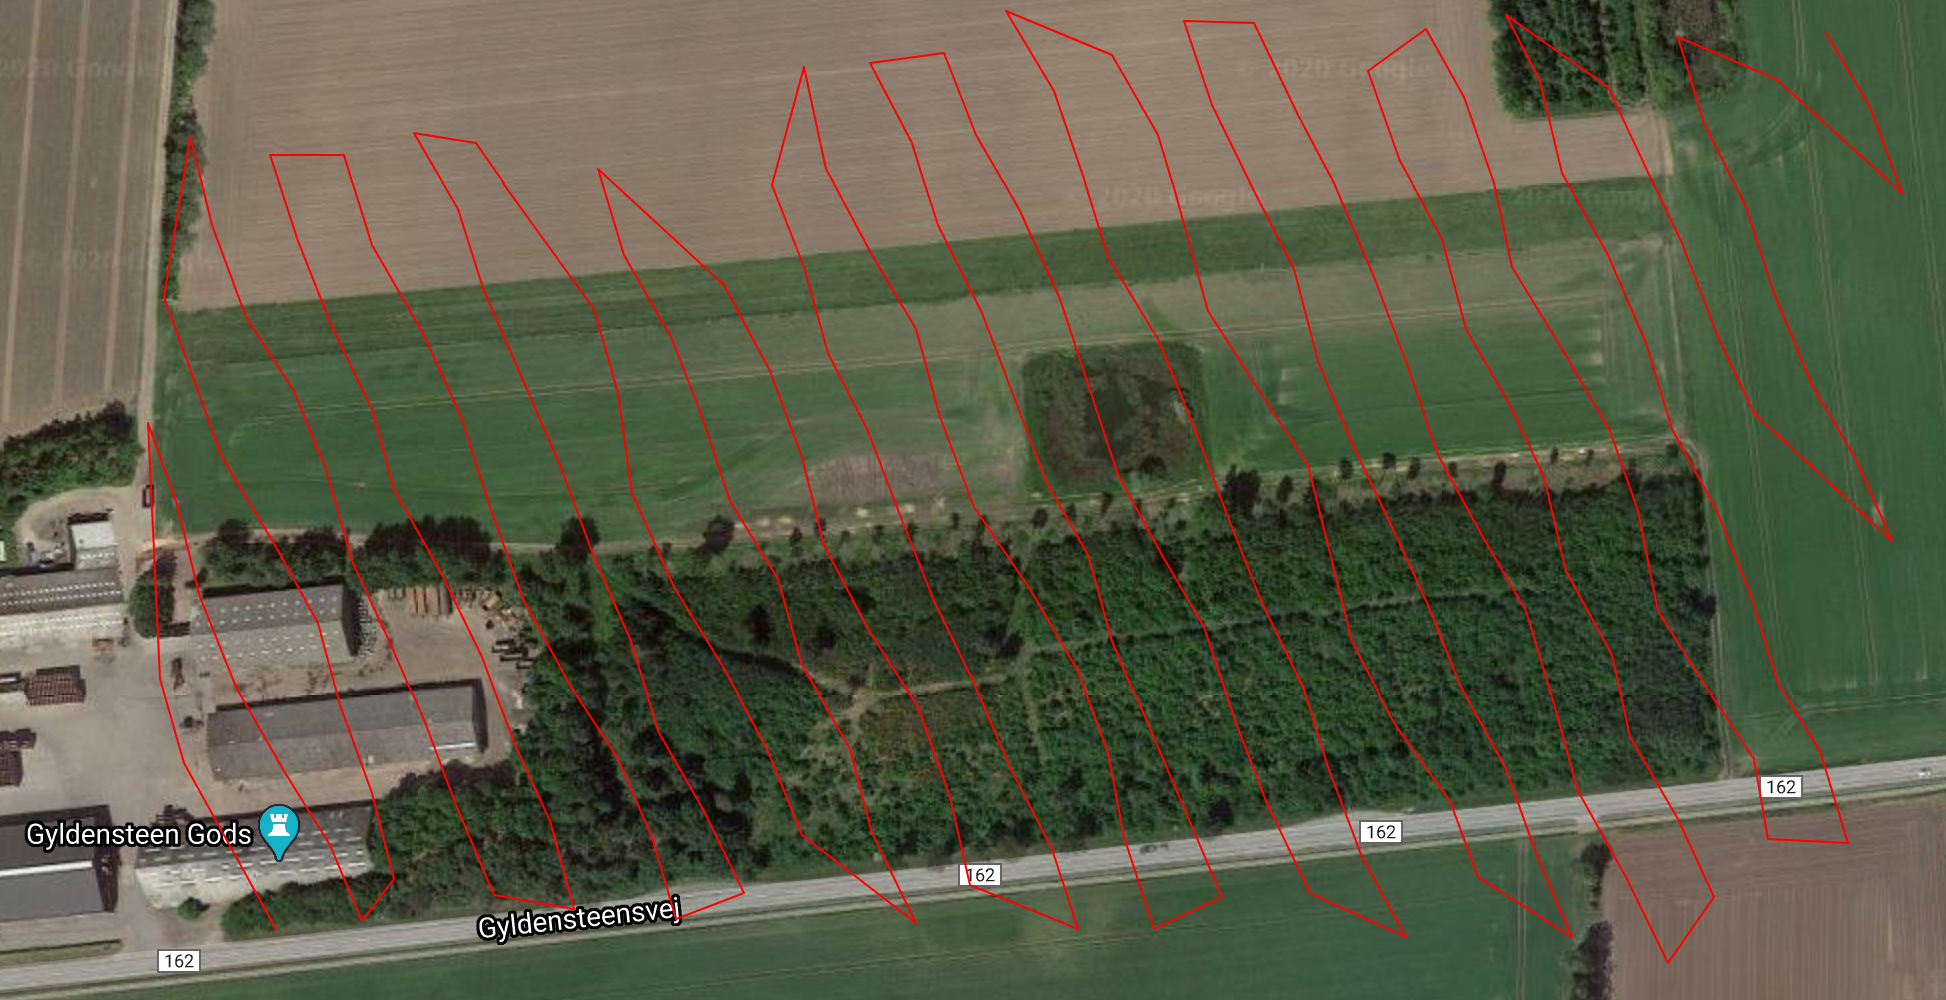
\includegraphics[width=0.75\textwidth]{../Figures/Flight_path}
	\caption{Illustration of the image path}
	\label{fig:flight_path}
\end{figure}

55.56666388888888 10.149922222222221\\
55.569547222222226 10.149922222222221\\
55.569547222222226 10.159333333333334\\
55.56666388888888 10.159333333333334\\

\end{itemize}


\end{document}